**intro**

\paragraph{Entry window}

\paragraph{Effect of radius}

Forfive different radii the dynamic pressure, Mach number and density that were encountered on a trajectory were recorded. For each radius an orbit for which the spacecraft just reaches the escape velocity and an orbit which decelerates as fast as possible while staying under 3g deceleration. The difference between these orbits indicates the maximal difference that can possibly be encountered.

\begin{figure}[H]
	\centering
	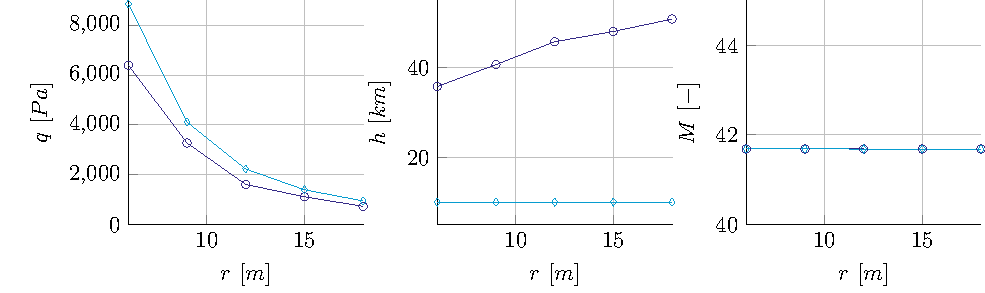
\includegraphics[width=1\textwidth]{./Figure/radius_param.pdf}
	\caption{maximal dynamic pressure, height and Mach number for different radii}
	\label{fig:radius}
\end{figure}

\paragraph{Effect of initial flight path angle}

\paragraph{Effect of angle of attack}

\paragraph{Effect of bank angle}



